\documentclass[11pt, a4paper]{report}

\usepackage{graphicx}
\graphicspath{ {images/} }

\usepackage{hyperref}
\usepackage[xindy]{glossaries}
\makeglossaries
\makeindex

\usepackage[utf8]{inputenc}
\usepackage{csquotes}


\begin{document}
\begin{titlepage}
	\title{IP6 - Report Street Networks} 
	\date{\today} 
	\author{J. Peyer, S. Merki} 
	\maketitle	
\end{titlepage}
\setcounter{page}{1}

\tableofcontents 



\begin{abstract}
	Text here.
\end{abstract}

\chapter{Introduction} 

\chapter{Theoretical Task} 
\section{Shape Grammar} 
The main key of shape grammar is to generate networks and paintings by a new defined grammar based on shape rules, selection rules, painting rules and limiting shapes. 
\newline
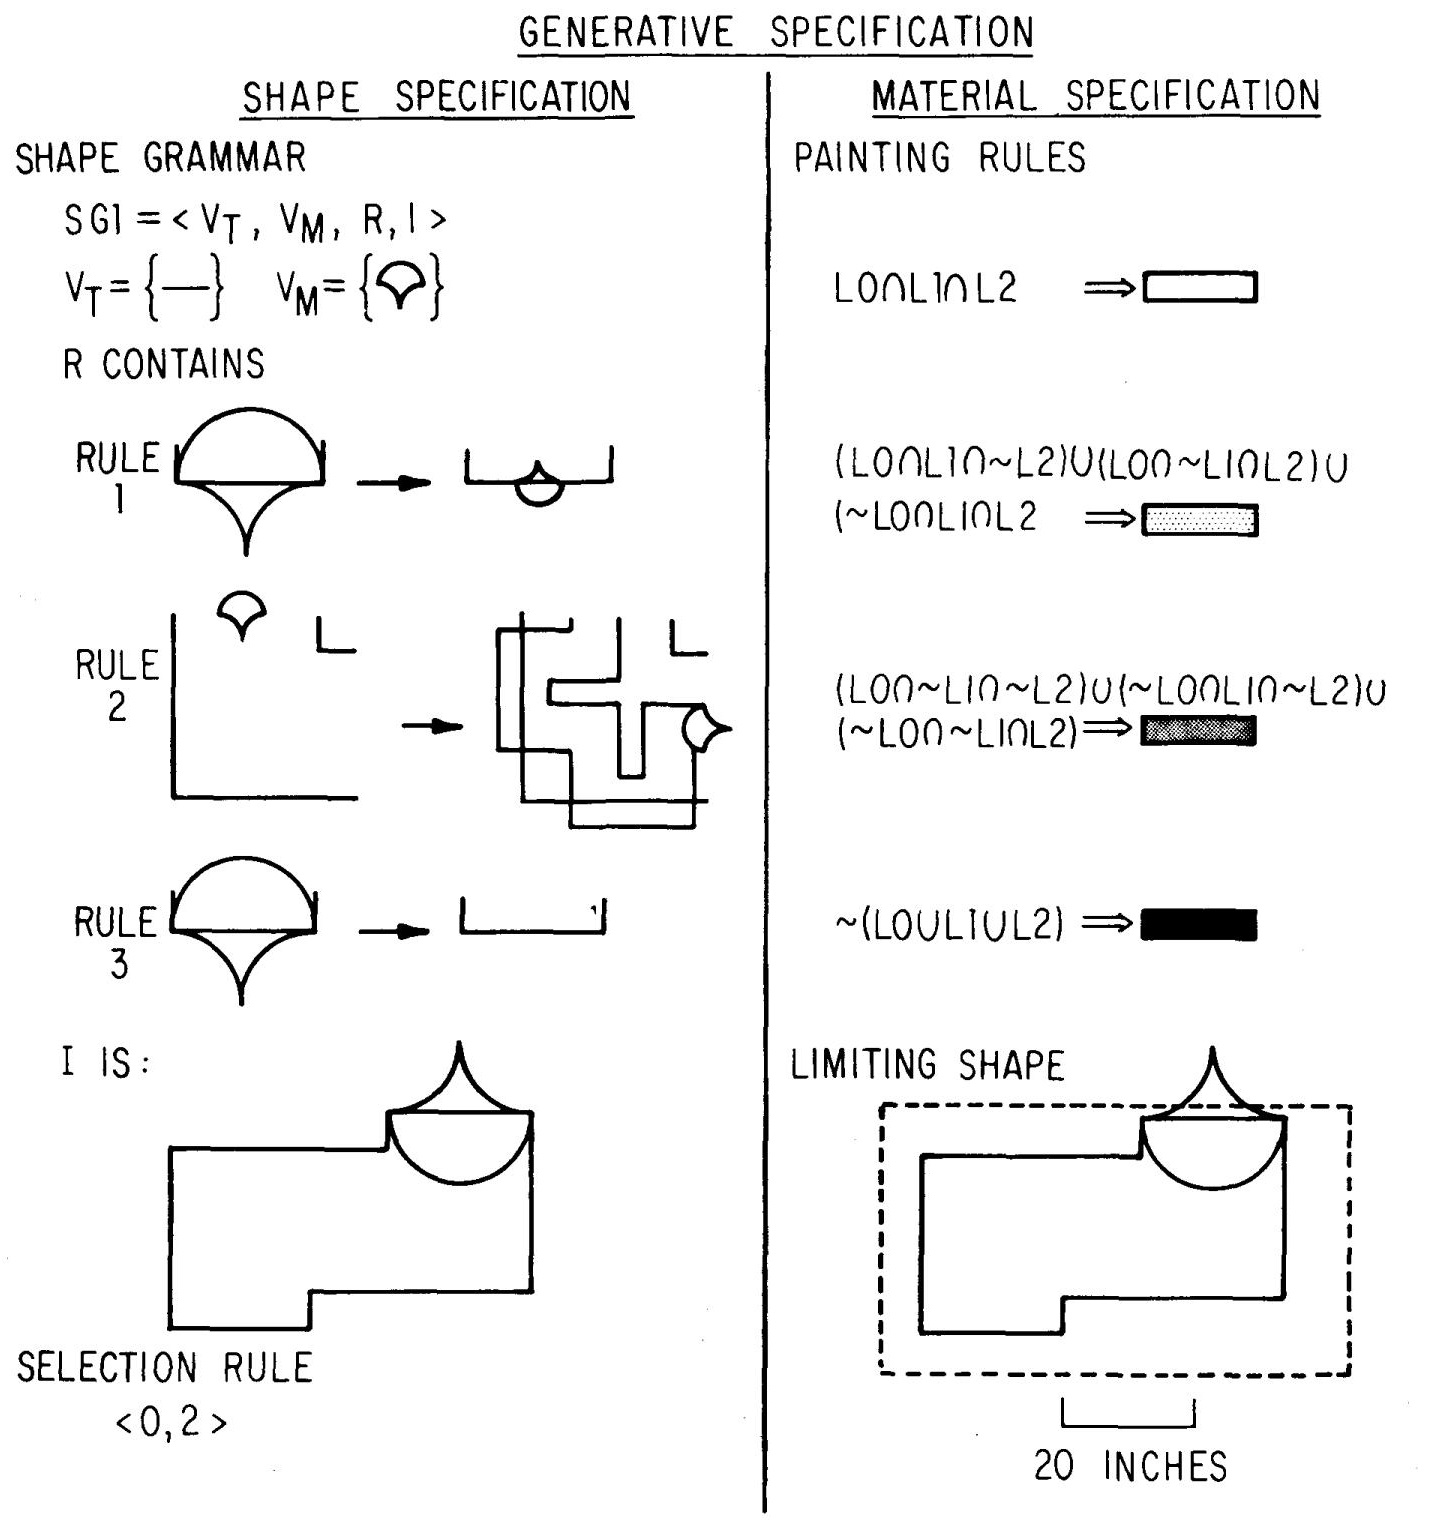
\includegraphics[scale=0.9]{generativ_specification}
\subsection{Shape Rules}


\subsection{Selection Rules}
An undefined count of shape rules provide the generation of the painting. Therefore a mechanism to select a correct shape is required.
Levels: During generation level's are assigned to the 
\begin{displayquote}
	\begin{enumerate}
		\item The terminals in the initial shape are assigned level 0.
		\item If a shape rule is applied, and the highest level assigned to any part ot the terminal corresponding to the level side of the rule is N, then
		\begin{enumerate}
			\item If the rule is of type A, any part of the terminal enclosed by the marker in the left side of the rule is assigned N.
			\item If the rule is of type B, any part of the terminal enclosed by the marker in the left side of the rule is assigned N and any part of the terminal enclosed by the marker is assigned N + 1.
			\item If the rule is of type C, the terminal added is assigned N + 1.
		\end{enumerate}
		\item No other level assignments are made.
	\end{enumerate}
\end{displayquote}
\subsection{Painting Rules}

\subsection{Limiting Shapes}
These Shapes define a limiting area of the canvas where shape painting is allowed. The area is normally defined as a rectangle, but this is not mandatory. 

\section{Procedural Modelling} 

\section{L-Systems}

\section{Extended L-Systems} 


\chapter{Practical Task} 

\section{CPlan}

\section{Graph to Tree}


\chapter{Conclusion}

\appendix
\glsaddall
\printglossaries
\end{document}